\begin{appendices}
%\addcontentsline{toc}{\chapter}{Appendices}
\appendixpage
\noappendicestocpagenum
\addappheadtotoc

\newcommand{\myWSEgPath}[1] {
\label{example:#1}
  \textcolor{blue} {(Please refer to .../workbooks/#1.nb)}}

\renewcommand{\thesection}{\arabic{section}}

\chapter*{Mathematica Workbook Listing}
~\\Here is a listing of most common seen heat transfer condition and regularly used methods for solving the problems. As listed, the problem marked with \textbf{*} were already mentioned in the tutorial examples. Others will be further discussed in the mathematica workbooks.

\section*{General topics}

\renewcommand{\labelitemiii}{$\circ$}

\begin{itemize}
\item Steady State: $\nabla^2T+\frac{\dot{q}}{k}=0$
\begin{itemize}
\item 1-D: Fourier's Law*
\item 1-D: Geometry: Cartesian*, Cylindrical, Spherical
\item 1-D: with heat generation
\item Special 1-D and Fin Solutions:
\begin{itemize}
\item Variable X-S area*
\item Fin: Cartesian*
\item Fin: Radial
\item Bioheat Equation (Fin analog)*
\end{itemize}
\end{itemize}

\item Multi-dimensional: $\nabla^2T+\frac{\dot{q}}{k}=0$
\begin{itemize}
\item 2-D: Exact solution rectangle*
\begin{itemize}
\item Derivative on a boundary (heat flux)*
\end{itemize}
\item NDSolve with heat generation
\end{itemize}

\item Transient: $\frac{1}{\alpha}\frac{\partial T}{\partial t}
=\nabla^2T+\frac{\dot{q}}{k}$
\begin{itemize}
\item Lumped form*
\begin{itemize}
\item Special case –radiative condition
\end{itemize}
\item Lumped vs. Transient one term solution*
\item SOV analytical solution*
\item NDSolve one dimensional with heat generation
\item Semi-infinite solutions
\end{itemize}


\item Numerical (Programming in Mathematica)
\begin{itemize}
\item Finite difference Fin*
\item Finite Difference Cartesian, Cylindrical and Spherical
\end{itemize}

\end{itemize}

\section*{Specific topics \uppercase\expandafter{\romannumeral1}}
\begin{itemize}
\item Multi-dimensional SOV solutions
\begin{itemize}
\item Cartesian
\item Cylindrical
\item Spherical
\end{itemize}

\item Laplace Solution
\item Duhamel
\item More Error Function Solutions
\end{itemize}

\section*{Specific topics \uppercase\expandafter{\romannumeral2}}
\begin{itemize}
\item Drug Delivery
\begin{itemize}
\item One compartment drug delivery
\item Two compartment drug delivery
\end{itemize}
\item Phase Change (Xiaoqing)
	\begin{itemize}
	\item Part \uppercase\expandafter{\romannumeral1}: Steady State
	\item Part \uppercase\expandafter{\romannumeral2}: Quasi – Steady Solutions (Cooper and Trezek)
	\item Part \uppercase\expandafter{\romannumeral3}: Neumann + Stefan
	\end{itemize}
\item Biophysics
	\begin{itemize}
	\item Arrhenius Modeling vs. Clinical Equivalent Minutes (CEM)
		\begin{itemize}
		\item Protein denaturation \& Fractional denaturation
		\item Thermal Dose
		\end{itemize}
	\item Water Transport
	\item Cryoprotective Loading
	\end{itemize}
\item Iron Oxide Nanoparticle Heating
	\begin{itemize}
	\item Cancer
	\item Regenerative Medicine (See Navid)
	\end{itemize}

\end{itemize}





\chapter{General Topics}
%\renewcommand{\thechapter}{\arabic{chapter}}

%\addcontentsline{titletoc}{part}{\appendixname}
\numberwithin{example}{section}
%\chapter{Workshops examples*}



\section{1-dimensional steady state}
\subsection{Variable heat generation}
\begin{example}
\textbf{1-D steady state solution in Cartisian coordinate}\\
BCs: at $x=0$, $T=10$; 
$x=1$, $T=100$ Heat Generation: g variable Given: $k=1$
\textcolor{blue} {\emph{Please refer to 1D Variheat Cati.nb}}
\begin{figure}[H]
  \centering
    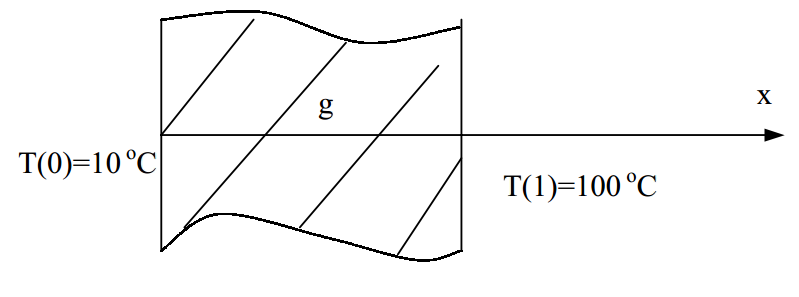
\includegraphics[scale=0.5]{figures/appendixA/1}
\end{figure}
$$T''+g=0$$
$$T=0.5gx^2+C_1x+C_2$$
\end{example}

\subsection{Spehrical coordinate}
\begin{example}
\textbf{1 - D steady state solution in spherical coordinate}\\
BCs: at $r = 0.1$, $T = 10$; $r = 1$, $T = 100$.
Heat Generation: g variable
Given: $k=1$ \textcolor{blue} {\emph{Please refer to 1D VariHeat spheri.nb}}
\begin{figure}[H]
  \centering
    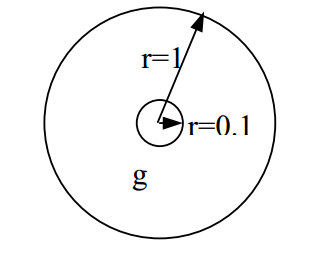
\includegraphics[scale=0.5]{figures/appendixA/2}
\end{figure}
$$\frac{1}{r}\frac{d^2}{dr^2}(rT)+g=0$$
$$T=\frac{1}{6}gr^2+\frac{C_1}{r}+C_2$$
\end{example}

\subsection{Round fin}
\begin{example}
\textbf{fin problem: round rod}\\
Given: $k=206W/m/K$
\textcolor{blue} {\emph{Please refer to Round fin.nb}}
\begin{figure}[H]
  \centering
    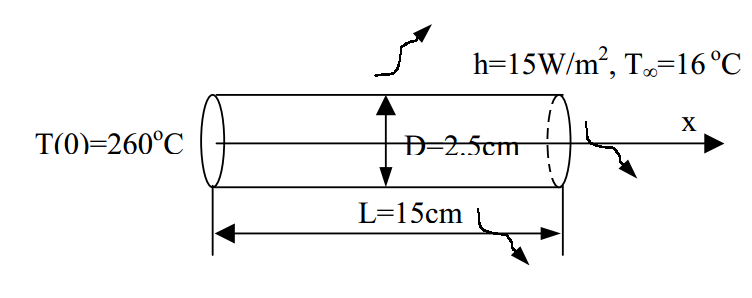
\includegraphics[scale=0.5]{figures/appendixA/3}
\end{figure}
$$\theta=T-T_\infty$$
$$\theta''-m^2\theta=0,~m=\sqrt{\frac{hp}{kA}}$$
$$\theta=\frac{\cosh{m(l-x)}+n\sinh{(m(l-x))}}{\cosh{(ml)}+n\sinh{(ml)}}\theta_0,~n=h/(km)$$
\end{example}

\section{Multi-dimensional steady state}
\subsection{2D square with heat generation}
\begin{example}
\textbf{NDSolve method}\textcolor{blue} {\emph{Please refer to 2D heat g NDSolve.nb}}
\end{example}

\section{Transient}
\subsection{Lumped form cylindrical}
\begin{example}
\textbf{lumped problem: long thin rod at $T(0)=20^oC$}\\
Given: $k = 0.5$; $\rho= 900$; $C_p = 3800$.
\textcolor{blue} {\emph{Please refer to lump long thin rod.nb}}
\begin{figure}[H]
  \centering
    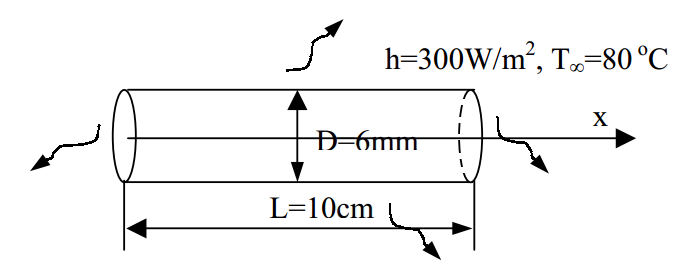
\includegraphics[scale=0.5]{figures/appendixA/4}
\end{figure}
$$\theta=T-T_\infty$$
$$\theta'-m^2\theta=0,~m=\sqrt{\frac{hA}{\rho C_pV}}$$
$$\theta=\theta_0e^{-mt}$$
\end{example}
\subsection{Lumped form radiative condition}
\begin{example}
A metal sphere of diameter $D$, which is at a uniform temperature $T_i$, is suddenly removed from a furnace and suspended from a fine wire in a large room with air at a uniform temperature $T_\infty$, and the surrounding walls are at a temperature $T_{surr}$.  
\textcolor{blue} {\emph{Please refer to Lumped with radiat.nb}}
\end{example}
\subsection{SOV method: Catesian, Cylindrical, Spherical}
\begin{example}
\textbf{ SOV (separation of variable) in 1D Cartisian space and time
No heat Generation}\\
$k = 0.5$; $\rho=1000$; $C_p = 4200$.
\textcolor{blue} {\emph{Please refer to SOV Carti.nb}}
\begin{figure}[H]
  \centering
    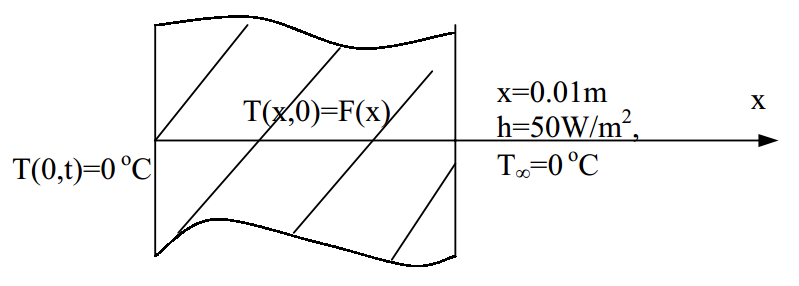
\includegraphics[scale=0.5]{figures/appendixA/5}
\end{figure}

$$\frac{\partial T}{\partial t}=
\alpha\left(\frac{\partial^2 T}{\partial x^2}+
\frac{\partial^2 T}{\partial y^2}+
\frac{\partial^2 T}{\partial z^2}\right)$$
$$T(x,t)=X(x)Y(y)Z(z)\Gamma(t)$$
$$X(x),~Y(y),~\text{and} ~Z(z)\text{: trigonometric function}$$
$$\Gamma(t)\text{: exponential decay function}$$
$$\text{Trigonometric differential equation: }X''+\beta^2X=0$$
$$T=\sum_{i=1}^{\infty} \frac{1}{N_i}e^{-\alpha{\beta_i}^2t}\sin{(\beta_i x)}\int_0^{l}\sin{(\beta_i x')}F(x')dx'$$
$$\beta\cot{(\beta l)}=-h/k$$
$$\frac{1}{N_i}=2\frac{{\beta_i}^2+{H_2}^2}{l({\beta_i}^2+{H_2}^2)+H_2},
~H_2=h/k$$
\end{example}
\begin{example}
\textbf{SOV (separation of variable) in 1D Cylindrical space and time
No heat Generation}
$k = 0.5$; $\rho= 1000$; $C_p = 4200$.
\textcolor{blue} {\emph{Please refer to SOV Cylin.nb}}
\begin{figure}[H]
  \centering
    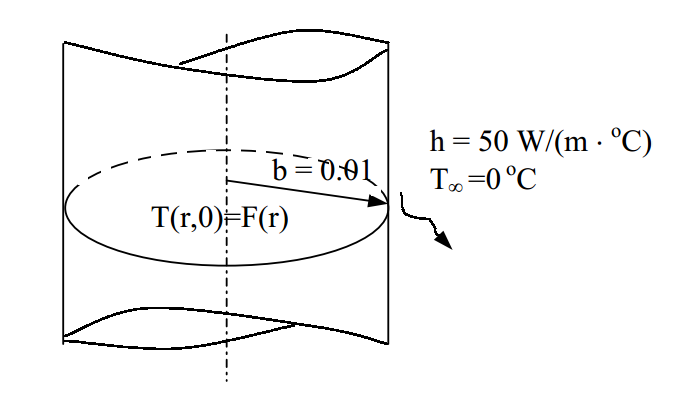
\includegraphics[scale=0.5]{figures/appendixA/6}
\end{figure}
$$\frac{1}{\alpha}\frac{\partial T}{\partial t}=
\frac{\partial^2 T}{\partial z^2}+
\frac{1}{r^2}\frac{\partial^2 T}{\partial \phi^2}+
\frac{1}{r}\frac{\partial T}{\partial r}+
\frac{\partial^2 T}{\partial r^2}$$
$$T(z,r,\phi,t)=Z(z)R(r)\Phi(\phi)\Gamma(t)$$
$$Z(z)~\text{and} ~\Phi(\phi)\text{: trigonometric}$$
$$R(r)\text{: Bessel function}$$
$$\Gamma(t)\text{: exponential decay function}$$
$$\text{Bessel differential equation (order } \upsilon\text{):}
\frac{\partial^2 R}{\partial r^2}+
\frac{1}{r}\frac{\partial R}{\partial r}+
\left(\beta^2-\frac{\upsilon^2}{r^2}\right) R=0
$$

$$\upsilon \text{ is eigenvalue of trigonometric differential equation of } \Phi(\phi)$$
$$T(r,t)=\sum_{i=1}^{\infty} \frac{1}{N_i}e^{-\alpha{\beta_i}^2t}J_\upsilon(\beta r)\int_0^{b}r'J_\upsilon(\beta r')F(r')dr'$$
$$0.5\beta(J_{\upsilon-1}(\beta b)-
J_{\upsilon+1}(\beta b))+
HJ_{\upsilon+1}(\beta b)=0,
~H=h/k
$$
$$\frac{1}{N_i}=\frac{2}{J_\upsilon(\beta b)}
\frac{\beta^2}{b^2(\beta^2+H^2)-\upsilon^2}
$$
\end{example}

\begin{example}
\textbf{SOV (separation of variable) in 1D spherical space and time: full sphere No heat Generation}\\
$k = 0.5$, $\rho= 1000$, $C_p = 4200$, $b=0.01$, $T(x,0)=60$, $T(b,t)=0$.
\textcolor{blue} {\emph{Please refer to SOV Spheri.nb}}
\begin{figure}[H]
  \centering
    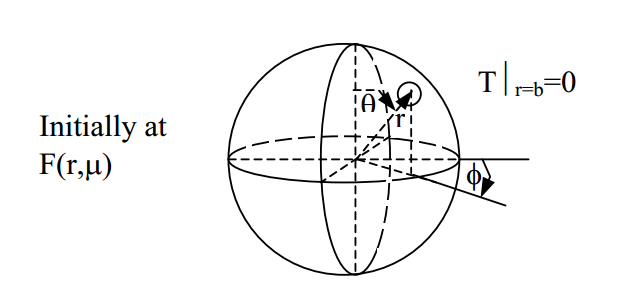
\includegraphics[scale=0.5]{figures/appendixA/7}
\end{figure}
$$ 
\frac{1}{\alpha}\frac{\partial T}{\partial t}=
\frac{\partial^2 T}{\partial r^2}+
\frac{2}{r}\frac{\partial T}{\partial r}+
\frac{1}{r^2\sin \theta} \frac{\partial}{\partial \theta}
\left( \sin\theta\frac{\partial T}{\partial \theta} \right)
+\frac{1}{r^2{\sin{\theta}}^2}\frac{\partial^2 T}{\partial \phi^2}
$$
$$\mu=\cos \theta,~V=r^{0.5}T$$
$$
\frac{1}{\alpha}\frac{\partial V}{\partial t}=
\frac{\partial^2 V}{\partial r^2}+
\frac{1}{r}\frac{\partial V}{\partial r}-
\frac{V}{4r^2}+
\frac{1}{r^2}\frac{\partial}{\partial \mu}
\left( (1-\mu^2)\frac{\partial V}{\partial \mu}\right)+
\frac{1}{r^2(1-\mu^2)}\frac{\partial^2 V}{\partial \phi^2}$$
$$V(r,\mu,\phi,t)=R(r)M(\mu)\Phi(\phi)\Gamma(t)$$
$$R(r)\text{: Bessel function, }\beta$$
$$\Phi(\phi)\text{: trigonometric, m}$$
$$\Gamma(t)\text{: exponential decay function}$$
$$M(\mu)\text{: Legendre polynomial}$$
$$ 
\frac{\partial^2 R}{\partial r^2}+
\frac{1}{r}\frac{\partial R}{\partial r}+
\left(\beta^2-\frac{(n+0.5)^2}{r^2}\right) R 
=0\text{, order n+0.5 Bessel differential equation}
$$
$$
\frac{\partial}{\partial \mu}
\left( (1-\mu^2)\frac{\partial V}{\partial \mu}\right)+
\left[ n(n+1)-\frac{m^2}{1-\mu^2} \right]M=0
$$
$$\text{Legendre’s associated differential equation of degree n and order m}$$

\begin{equation*}
\begin{aligned}
T(r,\mu,t)=&\sum_{n=0}^{\infty}\sum_{p=1}^{\infty} \frac{1}{N(n)N(\beta_{np})}
e^{-\alpha{\beta_{np}}^2t}r^{-0.5}J_{n+0.5}(\beta_{np}r)P_n(\mu)\times\\
&\int_{r'=0}^{b}\int_{\mu'=-1}^{1} {r'}^{1.5}J_{n+0.5}(\beta_{np}r')P_n(\mu')F(\mu',r')d\mu'dr'
\end{aligned}
\end{equation*}
$$J_{n+0.5}(\beta_{np}b)$$
$$N(n)=\frac{1}{2n+1}$$
$$N(\beta_{np})=-\frac{b^2}{2}J_{n-0.5}(\beta_{np}b)J_{n+1.5}(\beta_{np}b)$$
\end{example}

\begin{example}
\textbf{SOV (separation of variable) in 1D spherical space and time: half sphere}. \textcolor{blue} {\emph{Please refer to SOV half Spheri.nb}}
\begin{figure}[H]
  \centering
    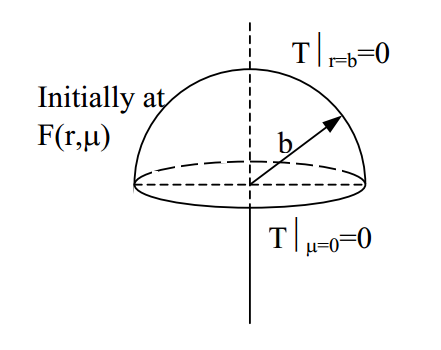
\includegraphics[scale=0.5]{figures/appendixA/8}
\end{figure}
\begin{equation*}
\begin{aligned}
T(r,\mu,t)=&\sum_{n=1,3,5\dots}^{\infty}\sum_{p=1}^{\infty} \frac{1}{N(n)N(\beta_{np})}
e^{-\alpha{\beta_{np}}^2t}r^{-0.5}J_{n+0.5}(\beta_{np}r)P_n(\mu)\times\\
&\int_{r'=0}^{b}\int_{\mu'=-1}^{1} {r'}^{1.5}J_{n+0.5}(\beta_{np}r')P_n(\mu')
F(\mu',r')d\mu'dr'
\end{aligned}
\end{equation*}

$$J_{n+0.5}(\beta_{np}b)$$
$$N(n)=\frac{1}{2n+1}$$
$$N(\beta_{np})=-\frac{b^2}{2}J_{n-0.5}(\beta_{np}b)J_{n+1.5}(\beta_{np}b)$$
\end{example}



\subsection{1-D with heat generation}
\begin{example}
\textbf{NDSolve 1-D heat generation} \textcolor{blue} {\emph{Please refer to 1-Dheatg ND.nb}}
\end{example}

\subsection{Semi-infinite solutions}
\begin{example}
\textbf{Semi-infinite domain solution: error function and complimentary error
function}\\
$k = 0.5$, $\rho= 1000$, $C_p = 4200$.
Initial condition: $T(x,0)=0$
Boundary condition: $T(0,t)=100^oC$ or convective $w/:h=100w/m^2$, $T_f=100^oC$.\textcolor{blue} {Please refer to error func semiinfi.nb}
\begin{figure}[H]
  \centering
    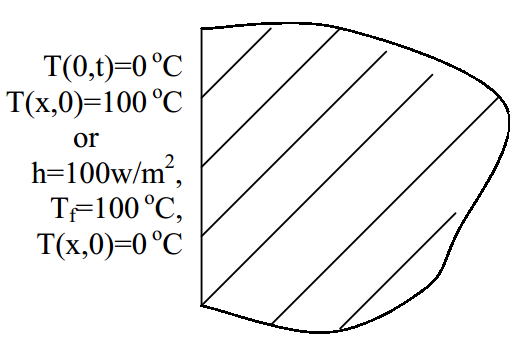
\includegraphics[scale=0.5]{figures/appendixA/9}
\end{figure}
$$T(x,t)=T_0 erf(x/\sqrt{4\alpha t}),~T(0,t)=0^o C\text{ or,}$$
\begin{eqnarray*}
&T(x,t)=T_0 erfc(x/\sqrt{4\alpha t})-e^{Hx+H^2\alpha t}
erfc(H \sqrt{\alpha t}+x\sqrt{4\alpha t})\\
&\text{ for convective conditions}
\end{eqnarray*}
\end{example}

\begin{example}
\textbf{Analytical solution}\textcolor{blue} {\emph{Please refer to f(t)semiinf.nb}}
\end{example}

\begin{example}
\textbf{Duhamel method}\textcolor{blue} {\emph{Please refer to Duhamelsemiinf.nb}}
\end{example}

\begin{example}
\textbf{Laplace method}\textcolor{blue} {\emph{Please refer to Laplace semiinf.nb}}
\end{example}

\subsection{Numerical method}
\begin{example}
\textbf{Finite Difference method for fin: Cartesian, Cylindrical and Spherical}\textcolor{blue} {\emph{Please refer to Fin Diff 3 Geometries.nb}}
\end{example}

\chapter{Special Topics \uppercase\expandafter{\romannumeral1}}
All the workbooks for problems listed in Appendix B Special Topics I could be found in \textcolor{blue} {\emph{Special Topic I.pdf}}
\section{Multi-dimensional SOV solutions}

\begin{example}
\textbf{Finite Difference method for fin: Cartesian, Cylindrical and Spherical}
\end{example}

\section{Laplace Solution}
\begin{example}
\textbf{Laplace Solution}
\end{example}

\section{Duhamel Solution}
\begin{example}
\textbf{Duhamel Solution}
\end{example}

\section{More Error Function Solutions}
\begin{example}
\textbf{Semi Infinite Domain}
\end{example}

\chapter{Special Topics \uppercase\expandafter{\romannumeral2}}

\section{Drug Delivery}
\begin{example}
\textbf{One compartment drug delivery}\textcolor{blue} {\emph{Please refer to one-comp drug deli.nb}}
\end{example}

\begin{example}
\textbf{Two compartment drug delivery}\textcolor{blue} {\emph{Please refer to two-comp drug deli.nb}}
\end{example}

\section{Phase Change}
\begin{example}
\textbf{Part I: Steady State}\textcolor{blue} {\emph{Please refer to Phase Change Problems.nb}}
\end{example}

\begin{example}
\textbf{Part II: Quasi – Steady Solutions (Cooper and Trezek)}\textcolor{blue} {\emph{Please refer to Phase Change Problems.nb}}
\end{example}

\begin{example}
\textbf{Part III:  Neumann + Stefan}\textcolor{blue} {\emph{Please refer to Phase Change Problems.nb}}
\end{example}

\section{Biophysics}
\subsubsection{Arrhenius Modeling vs. Clinical Equivalent Minutes (CEM)}
\begin{example}
\textbf{Protein denaturation \& Fractional denaturation}\textcolor{blue} {\emph{Please refer to CPALoading2012v042914.nb, CPALoadWeiss.nb, CPALoadingSmith.nb}}
\end{example}

\begin{example}
\textbf{Thermal Dose}\textcolor{blue} {\emph{Please refer to Thermal Dose.nb }}
\end{example}

\subsection{Water Transport}
\begin{example}
\textbf{Water Transport Simulation}\textcolor{blue} {\emph{Please refer to Water Trans.nb}}
\end{example}
\subsection{Cryoprotective Loading}


\section{Iron Oxide Nanoparticle Heating}

\begin{example}
\textbf{Cancer}\textcolor{blue} {\emph{Please refer to FEO NP for Cancer Treat.nb}}
\end{example}

\begin{example}
\textbf{Regenerative Medicine}
\end{example}

\end{appendices}
